\documentclass[tcc]{ic}

\hypersetup{
    colorlinks = {true},
    linktocpage = {false},
    plainpages = {false},
    linkcolor = {Blue},
    citecolor = {Blue},
    urlcolor = {Red},
    unicode = {true},
    pdftitle = {Gerando interfaces nativas para desktop com código único},
    pdfauthor = {Eduardo Maciel Alexandre},
    pdfsubject = {Trabalho de Conclusão de Curso},
    pdfkeywords = {desenvolvimento multiplataforma, interfaces nativas, geração de código, transpilação, cross-platform development, native user interfaces, code generation, transpilation}
}

\usepackage{algorithm}
\usepackage{algpseudocode}
\usepackage{tabularx}
\usepackage{array}

\makeatletter
\renewcommand{\ALG@name}{Algoritmo}
\renewcommand{\listalgorithmname}{List of \ALG@name s}
\makeatother

\newcolumntype{Y}{>{\centering\arraybackslash}X}

% Marcador visível para pontos que precisam de confirmação
\newcommand{\todo}[1]{\textcolor{red}{\textbf{[#1]}}}

\begin{document}

    % Inclui o preâmbulo do documento (Informações da capa e contracapa)
    \titulo{Gerando interfaces nativas para desktop com código único}

\autor{Eduardo Maciel Alexandre}{ema2@ic.ufal.br}{https://theduardomaciel.vercel.app/}

\orientador{Prof. Dr. Fábio José Coutinho da Silva}{}{Instituto de Computação}{Universidade Federal de Alagoas}{}

% \examinador{Nome}{}{Instituto de Computação}{Universidade Federal de Alagoas}{Prof. Me.}

% \examinadorDois{Nome}{}{Instituto de Computação}{Universidade Federal de Alagoas}{Prof. Me.}

\dataMesAno{Novembro}{2026}{}

    \selectlanguage{portuguese}
    
    % Capa, contracapa e avaliadores
    \capa
    
    % Agradecimentos
    %\begin{agradecimentos}

Obrigado

\end{agradecimentos}
    
    % Resumo e Abstract
    \begin{resumo}
    Frameworks multiplataforma reduzem a duplicação de código, mas costumam cobrar em desempenho e consumo de recursos. Além disso, muitos renderizam a própria interface ou embutem uma WebView, o que compromete a aderência ao design system de cada sistema operacional. Manter uma versão nativa por plataforma evita esses custos, mas multiplica as bases de código. Este trabalho propõe gerar, a partir de uma única fonte declarativa, projetos nativos para Windows (WinUI~3) e macOS (SwiftUI), sem camada de renderização própria. O objetivo é avaliar se as aplicações geradas atingem desempenho comparável ao de aplicações escritas à mão nas ferramentas oficiais de cada plataforma e em que medida a fonte única consegue expressar os componentes de interface de cada sistema. Para isso, um experimento compara três versões de duas aplicações de referência (nativa escrita à mão, gerada e com renderização própria) em tempo de resposta, memória, CPU, armazenamento e similaridade visual.

    \palavrasChave{desenvolvimento multiplataforma; interfaces nativas; geração de código; transpilação; desempenho;}
\end{resumo}

    \begin{abstract}
    Cross-platform frameworks reduce code duplication, but they usually cost performance, resources and fidelity to each operating system's design. Recent work on deterministic transpilation brings native development closer to a shared codebase, but targets Android and iOS and leaves the user interface in the background. In the literature examined, no study was found that generates native desktop interfaces (Windows and macOS) from a single source and evaluates the result. This work aims to evaluate whether applications generated from a single source, with native projects per operating system, achieve performance comparable to applications handwritten with each platform's official tools. The evaluation compares three versions of two reference applications (handwritten native, generated and self-rendered) in response time, memory, CPU, storage and visual similarity.

    \keywords{cross-platform development; native user interfaces; code generation; transpilation; performance;}
\end{abstract}


    % Declaração de uso de IA
    %\chapter*{\thispagestyle{empty}\centering Declaração de uso de IA}
\onehalfspacing
\todo{rascunho; confirmar e corrigir cada item}

\textbf{Ferramenta e versão.} Claude (Anthropic), com o modelo \todo{Claude Sonnet 5.5? conferir a versão usada}.

\textbf{Para que usei.} Sugestões de título, de hipóteses e de estrutura do texto, montagem do projeto em LaTeX e redação de uma primeira versão das seções, a partir dos artigos da minha revisão bibliográfica e dos slides da disciplina.

\textbf{O que aproveitei e o que descartei.} \todo{descrever o que foi mantido, o que descartado e por quê}

\textbf{Verificação.} \todo{listar as obras que li integralmente e as que só conhece pelo resumo; ex.: GUIMigrator, SequalsK, Mahmoud et al.\ e Biørn-Hansen et al.\ foram lidos na íntegra}


    % Sumário
    \tableofcontents
    \thispagestyle{empty}
    
    % Início dos capítulos
    \inicio
    
    \mychapter{Introdução}{cap:introducao}
\lhead{INTRODUÇÃO}

Construir a interface de usuário está entre as tarefas mais custosas do desenvolvimento de aplicações móveis, a ponto de consumir mais da metade do esforço total \cite{gao2026guimigrator}. Manter uma versão nativa por plataforma multiplica esse custo, pois exige equipes e bases de código separadas. Por isso, a demanda por soluções eficientes e de baixo custo impulsionou a adoção de frameworks multiplataforma \cite{jost2025state}. Esses frameworks reduzem a duplicação, mas cobram em desempenho e uso de recursos e criam forte dependência da ferramenta \cite{biorn2020empirical, mahmoud2024trans, schultes2025native}. Em uma comparação empírica, Biørn-Hansen et al.\ mediram CPU, memória e tempo de resposta de cinco frameworks e de uma implementação nativa e concluíram que o desempenho multiplataforma é, em geral, inferior ao nativo, sem que nenhum framework seja o pior ou o melhor em todas as métricas \cite{biorn2020empirical}.

Abordagens recentes substituem a camada intermediária por transpilação determinística. O SequalsK compartilha a camada de modelo entre Kotlin e Swift e permite escrever até 86\% do código uma única vez, mas não cobre a interface, que os próprios autores deixam como trabalho futuro \cite{schultes2025native}. O GUIMigrator converte interfaces Android em XML para Jetpack Compose e SwiftUI, com similaridade visual média de 81,9\% e 78,2\%, respectivamente \cite{gao2026guimigrator}. Mahmoud et al.\ convertem aplicações React Native e Xamarin em aplicações nativas, que superaram as originais em memória, armazenamento e velocidade \cite{mahmoud2024trans}. Na literatura triada, os três trabalhos têm Android e iOS como alvo e nenhum gera interfaces nativas de desktop (Windows e macOS) a partir de uma fonte única. No desktop, os estudos encontrados tratam dos desafios de aplicações baseadas em web view \cite{scoccia2021challenges} e da comparação entre Electron, Tauri e PyQt quanto à integração com o sistema, à memória e ao tamanho do instalador \cite{milichiewicz2025comparative}.

Diante dessa lacuna, este trabalho tem como objetivo avaliar se a geração de projetos nativos para cada sistema operacional (SwiftUI no macOS e WinUI no Windows) a partir de uma única fonte produz aplicações com desempenho comparável e alta similaridade visual em relação às escritas diretamente nas ferramentas oficiais de cada plataforma, sem a camada de renderização própria dos frameworks atuais.

    % \include{capitulos/fundamentacao}
    % \mychapter{Materiais e Métodos}{cap:metodos}
\lhead{MATERIAIS E MÉTODOS}

A pesquisa é aplicada e experimental. Duas aplicações de referência, com telas de lista, formulário e navegação, serão projetadas no Figma com as bibliotecas oficiais de componentes de cada sistema operacional e implementadas em três versões: (A) escrita à mão em SwiftUI (macOS) e WinUI~3 (Windows); (B) gerada pelo framework a partir de uma fonte única; (C) com renderização própria, usando Electron como \textit{baseline}, um dos frameworks avaliados no desktop por Milichiewicz e Badurowicz \cite{milichiewicz2025comparative}. As três versões partem do mesmo projeto no Figma.

O framework será desenvolvido de forma iterativa. A fonte única será escrita em Kotlin, com sintaxe declarativa, e o gerador, preferencialmente em Rust, a lerá por análise sintática (parser externo ou plugin do compilador Kotlin, a definir) e produzirá os projetos nativos. O escopo se restringe a aplicações simples para Windows e macOS, e o Linux será tratado como trabalho futuro.

As medidas de desempenho são uso de CPU, memória e tempo de resposta, como em Biørn-Hansen et al.\ \cite{biorn2020empirical}, mais tamanho de armazenamento, como em Mahmoud et al.\ \cite{mahmoud2024trans}. Cada medição será repetida o suficiente para reportar mediana, intervalo de confiança e tamanho de efeito, e a H1 será avaliada por um teste de equivalência (como o TOST), com a margem fixada antes da coleta. A fidelidade visual será medida por similaridade estrutural (SSIM) entre capturas de tela das versões geradas e das escritas à mão, métrica também usada no GUIMigrator \cite{gao2026guimigrator}, e a cobertura de componentes nativos, por lista de conferência.

Os experimentos rodarão em uma máquina com macOS e em outra com Windows 11, ambas com hardware e versão do sistema mantidos fixos durante toda a coleta. Cada sistema será medido com as ferramentas de \textit{profiling} da própria plataforma, e as três versões rodarão nas mesmas condições (mesmo equipamento, mesma carga e estado inicial limpo). Todo o código, as telas de referência e os dados coletados ficarão no repositório do trabalho, para que a comparação possa ser replicada.

    % \include{capitulos/resultados_experimentais}
    %\mychapter{Conclusão}{cap:conclusao}
\lhead{CONCLUSÃO}

Lorem ipsum dolor sit amet, consectetur adipiscing elit. Duis elit tellus, vehicula in justo eget, fermentum aliquet nisi. In id quam mauris. Sed id vehicula libero. Quisque id tortor placerat, consequat ex sed, placerat ante. Ut dui nunc, placerat volutpat ipsum sit amet, dictum pellentesque lacus. Donec leo sem, dictum quis lacus at, ultricies sagittis elit. Mauris sit amet tortor efficitur, luctus justo sit amet, tincidunt tellus. Donec vulputate non risus at tincidunt. Sed accumsan at erat in aliquet. Sed consequat gravida bibendum. Sed fermentum metus sed ex lacinia mattis. Phasellus vel enim nisl. Proin tortor dui, luctus in erat a, dapibus convallis turpis. Maecenas vitae vulputate neque.

\section{Seção}

Etiam ac ante a lorem consectetur varius. Donec vitae dui porttitor, efficitur ante sed, aliquet lectus. Etiam aliquet mattis sagittis. Integer accumsan, est nec vehicula suscipit, nibh nisl varius ante, at convallis urna est dapibus massa. Orci varius natoque penatibus et magnis dis parturient montes, nascetur ridiculus mus. Praesent tempus dolor sit amet metus eleifend porta. Vestibulum eget viverra nulla. Mauris ac condimentum augue, quis molestie tortor. Duis ac condimentum tortor, sed ullamcorper nunc. Vivamus et suscipit arcu. Duis eget rutrum est, sed pellentesque leo. Nulla lorem lacus, faucibus vitae lectus eu, porttitor efficitur ante. Sed risus tortor, venenatis quis convallis non, blandit in orci. Morbi et neque hendrerit, consectetur magna vitae, consectetur dolor. Nam nec iaculis urna, vitae tincidunt eros. Ut pretium neque convallis turpis rutrum, nec dapibus est faucibus.

\begin{figure}[H]
    \centering
    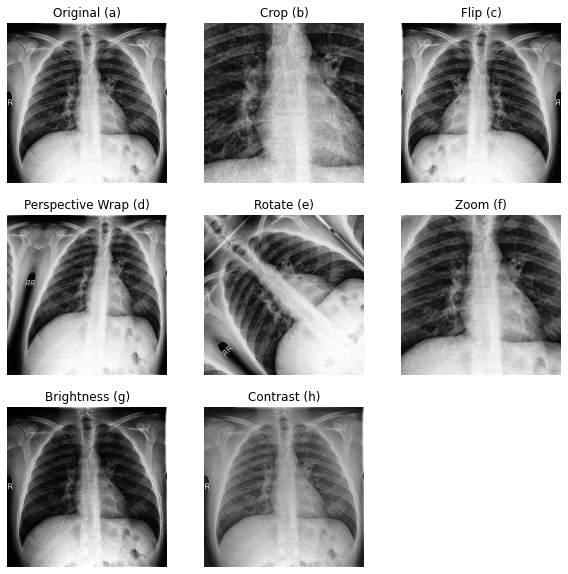
\includegraphics[width=\textwidth - \textwidth / 6]{res/intro/tfms.png}
    \caption{Legenda}
    \label{fig:tfms_examples}
\end{figure}

Agora um monte de referência, \cite{tanner1987calculation, eaton2018improving}


    \mychapter{Objetivos}{cap:objetivos}
\lhead{OBJETIVOS}

\textbf{Objetivo geral.} Avaliar se aplicações geradas a partir de uma fonte única, com projetos nativos por sistema operacional, atingem desempenho comparável ao de aplicações escritas à mão nas ferramentas nativas de Windows e macOS.

\textbf{Objetivos específicos.}
\begin{enumerate}
  \item Quantificar a diferença de desempenho (tempo de resposta, memória e CPU) entre as aplicações geradas e as escritas à mão.
  \item Comparar as aplicações geradas com uma versão de renderização própria.
  \item Medir a similaridade visual das aplicações geradas em relação às escritas à mão.
  \item Determinar a fração dos componentes de interface de cada sistema operacional que a fonte única consegue expressar.
\end{enumerate}

\textbf{Pergunta de pesquisa.} Como desenvolver aplicativos multiplataforma que fazem uso dos componentes nativos de interface em uma base única de código, sem perda de desempenho em relação ao desenvolvimento nativo?

\textbf{Hipóteses.} Formuladas antes dos experimentos, H1 a H3 competem entre si.
\begin{itemize}
  \item \textbf{H1:} as aplicações geradas têm desempenho equivalente ao das escritas à mão, isto é, a diferença entre as medianas fica dentro de uma margem de equivalência pré-definida.
  \item \textbf{H2:} as aplicações geradas têm desempenho superior ao da versão com renderização própria, tanto no Windows quanto no macOS.
  \item \textbf{H3 (rival):} o custo da geração e da camada compartilhada anula o ganho, e as aplicações geradas ficam equivalentes à versão com renderização própria.
  \item \textbf{H4 (cobertura):} a fonte única não cobre todos os componentes nativos do Windows e macOS, e a similaridade visual (SSIM) é menor nas telas com componentes não cobertos.
\end{itemize}

    \mychapter{Relevância do Trabalho}{cap:relevancia}
\lhead{RELEVÂNCIA DO TRABALHO}

A contribuição principal recai sobre a computação, e não sobre o domínio das aplicações de exemplo. O trabalho leva para o desktop a pergunta que SequalsK e GUIMigrator respondem apenas para Android e iOS e busca endereçar uma limitação que o próprio SequalsK aponta: a tradução da camada de interface, que limitou o código compartilhado a 16\% em um dos seus estudos de caso \cite{schultes2025native}. Na literatura triada, há uma lacuna de contexto (poucas avaliações em desktop com interface nativa) e metodológica, pois as comparações de desempenho e os estudos de tendências encontrados tratam de frameworks móveis \cite{biorn2020empirical, jost2025state}.

O trabalho entrega evidência empírica sobre três abordagens avaliadas nas mesmas aplicações de referência: código nativo escrito à mão, geração a partir de fonte única e abordagem multiplataforma convencional. Para desenvolvedores que valorizam desempenho e aderência ao design de cada sistema, os resultados ajudam a decidir entre manter uma base de código por sistema, com custo alto, e adotar um framework multiplataforma, com interface que destoa da plataforma. Na abordagem proposta, por gerar projetos nativos padrão, o código permanece inspecionável em cada sistema, o que tende a reduzir o aprisionamento a uma camada opaca.

O trabalho também adota geração determinística, em contraste com a migração por modelos de linguagem. Tanto o GUIMigrator quanto o conversor de Mahmoud et al.\ relatam resultados superiores aos de \textit{baselines} baseados em LLMs \cite{gao2026guimigrator, mahmoud2024trans}. A geração de interfaces a partir de modelos já é uma linha estabelecida \cite{ruiz2019evaluating}, e aqui ela é aplicada à produção de componentes nativos de desktop.

No contexto de desktop, estudos comparativos como o de Milichiewicz e Badurowicz avaliam ferramentas multiplataforma (Electron, Tauri e PyQt) entre si e apontam compromissos de integração com o sistema e consumo de recursos \cite{milichiewicz2025comparative}, mas não incluem uma versão nativa desenvolvida manualmente como \textit{baseline}. A novidade, portanto, está na combinação de geração a partir de fonte única, interface nativa de desktop e comparação com o código nativo.

O trabalho é viável no prazo, pois o escopo se restringe a aplicações simples para Windows e macOS, há equipamentos disponíveis e o projeto das aplicações dispensa dados externos.
    \mychapter{Materiais e Métodos}{cap:metodos}
\lhead{MATERIAIS E MÉTODOS}

A pesquisa é aplicada e experimental. Duas aplicações de referência, com telas de lista, formulário e navegação, serão projetadas no Figma com as bibliotecas oficiais de componentes de cada sistema operacional e implementadas em três versões: (A) escrita à mão em SwiftUI (macOS) e WinUI~3 (Windows); (B) gerada pelo framework a partir de uma fonte única; (C) com renderização própria, usando Electron como \textit{baseline}, um dos frameworks avaliados no desktop por Milichiewicz e Badurowicz \cite{milichiewicz2025comparative}. As três versões partem do mesmo projeto no Figma.

O framework será desenvolvido de forma iterativa. A fonte única será escrita em Kotlin, com sintaxe declarativa, e o gerador, preferencialmente em Rust, a lerá por análise sintática (parser externo ou plugin do compilador Kotlin, a definir) e produzirá os projetos nativos. O escopo se restringe a aplicações simples para Windows e macOS, e o Linux será tratado como trabalho futuro.

As medidas de desempenho são uso de CPU, memória e tempo de resposta, como em Biørn-Hansen et al.\ \cite{biorn2020empirical}, mais tamanho de armazenamento, como em Mahmoud et al.\ \cite{mahmoud2024trans}. Cada medição será repetida o suficiente para reportar mediana, intervalo de confiança e tamanho de efeito, e a H1 será avaliada por um teste de equivalência (como o TOST), com a margem fixada antes da coleta. A fidelidade visual será medida por similaridade estrutural (SSIM) entre capturas de tela das versões geradas e das escritas à mão, métrica também usada no GUIMigrator \cite{gao2026guimigrator}, e a cobertura de componentes nativos, por lista de conferência.

Os experimentos rodarão em uma máquina com macOS e em outra com Windows 11, ambas com hardware e versão do sistema mantidos fixos durante toda a coleta. Cada sistema será medido com as ferramentas de \textit{profiling} da própria plataforma, e as três versões rodarão nas mesmas condições (mesmo equipamento, mesma carga e estado inicial limpo). Todo o código, as telas de referência e os dados coletados ficarão no repositório do trabalho, para que a comparação possa ser replicada.

    \mychapter{Cronograma}{cap:cronograma}
\lhead{CRONOGRAMA}

A definição do tema e do problema e a triagem da literatura já foram concluídas. As etapas restantes estão distribuídas, em estimativa mensal, ao longo dos próximos semestres. \todo{ajustar os meses ao calendário real e ao prazo de entrega do TCC}

\begin{table}[H]
\centering
\footnotesize
\setlength{\tabcolsep}{3pt}
\begin{tabular}{@{}p{6.2cm}ccccccccc@{}}
\toprule
Etapa & \rotatebox{90}{Dez/26} & \rotatebox{90}{Jan/27} & \rotatebox{90}{Fev/27} & \rotatebox{90}{Mar/27} & \rotatebox{90}{Abr/27} & \rotatebox{90}{Mai/27} & \rotatebox{90}{Jun/27} & \rotatebox{90}{Jul/27} & \rotatebox{90}{Ago/27} \\
\midrule
Revisão bibliográfica e refino do objetivo & X & X & & & & & & & \\
Projeto das aplicações de referência (Figma) & X & X & & & & & & & \\
Desenvolvimento do gerador & & X & X & X & X & & & & \\
Implementação das três versões das aplicações & & & & X & X & X & & & \\
Experimentos e coleta de dados & & & & & & X & X & & \\
Análise e discussão dos resultados & & & & & & & X & X & \\
Redação e revisão com o orientador & X & X & X & X & X & X & X & X & X \\
Apresentação final & & & & & & & & & X \\
\bottomrule
\end{tabular}
\end{table}

    
    % Pós Textuais
    %\nocite{*}
    % Referências Biliográficas
\begin{raggedright}
\bibliographystyle{plainnat}
\renewcommand{\bibsection}{
\chapter*{\begin{flushright}Referências bibliográficas\end{flushright}}
\addcontentsline{toc}{chapter}{Referências bibliográficas}
}
\lhead{REFERÊNCIAS BIBLIOGRÁFICAS}
\bibliography{referencias}
\newpage\lhead{\rightmark}
\end{raggedright}

% As referências estão no arquivo referencias.bib

\end{document}
